%%%%%%%%%%%%%%%%%%%%%%% file typeinst.tex %%%%%%%%%%%%%%%%%%%%%%%%%
%
% This is the LaTeX source for the instructions to authors using
% the LaTeX document class 'llncs.cls' for contributions to
% the Lecture Notes in Computer Sciences series.
% http://www.springer.com/lncs       Springer Heidelberg 2006/05/04
%
% It may be used as a template for your own input - copy it
% to a new file with a new name and use it as the basis
% for your article.
%
% NB: the document class 'llncs' has its own and detailed documentation, see
% ftp://ftp.springer.de/data/pubftp/pub/tex/latex/llncs/latex2e/llncsdoc.pdf
%
%%%%%%%%%%%%%%%%%%%%%%%%%%%%%%%%%%%%%%%%%%%%%%%%%%%%%%%%%%%%%%%%%%%

%\documentclass[runningheads,a4paper]{llncs}
\documentclass[a4paper]{llncs}

%\usepackage{amssymb}
%\setcounter{tocdepth}{3}
%\usepackage{graphicx}
\usepackage{url}
\usepackage[utf8]{inputenc}
\usepackage{todonotes}
%\usepackage{hyperref}
%\usepackage{booktabs}
%\usepackage{subfig}
%\usepackage{array}
\usepackage[portuges]{babel}

% \newcommand{\papertitle}{A Distributed Computing Framework for Heterogeneous Environments}


\newcommand{\papertitle}{PCap com filtragem orientada ao processo}

%\newcommand{\papertitle}{Leveraging GPUs for Scientific Computing}

%\hypersetup{pdfborder=0 0 0,
%            pdfauthor={Nuno Martins \and Vítor Duarte},
%%            pdfcreator=,
%            pdfkeywords={Pcap, linux, monitorização,},
%%            pdfsubject=TesteSubject,
%            pdftitle={\papertitle}
%           }


\urldef{\mailsa}\path|nuno.m.g.martins@gmail.com|
\urldef{\mailsb}\path|vad@di.fct.unl.pt|    

\newcommand{\keywords}[1]{\par\addvspace\baselineskip
\noindent\keywordname\enspace\ignorespaces#1}

\newcommand{\td}[1]{\todo[inline]{#1}}


\begin{document}

\mainmatter  % start of an individual contribution

% first the title is needed
\title{\papertitle}

\author{Nuno Martins\inst{1} e Vítor Duarte\inst{2}}
%
\authorrunning{\papertitle}
% (feature abused for this document to repeat the title also on left hand pages)

% the affiliations are given next; don't give your e-mail address
% unless you accept that it will be published
\institute{\email{nuno.m.g.martins@gmail.com} \and \email{vad@di.fct.unl.pt}\\
CITI --- Departamento de Informática,\\
Faculdade de Ciências e Tecnologia,\\
Universidade Nova de Lisboa, Portugal}
%\mailsa \qquad \mailsb}

%
% NB: a more complex sample for affiliations and the mapping to the
% corresponding authors can be found in the file "llncs.dem"
% (search for the string "\mainmatter" where a contribution starts).
% "llncs.dem" accompanies the docume\label{•} nt class "llncs.cls".
%

%\toctitle{Lecture Notes in Computer Science}
%\tocauthor{Authors' Instructions}
\maketitle

\begin{abstract}

A monitorização do comportamento dos processos é uma das melhores formas de compreender a sua execução real, de detectar erros e avaliar o seu real desempenho, ainda mais se não for possível aceder ao seu código fonte. No entanto, o impacto no desempenho e comportamento das aplicações pode ser bastante significativo.
 O caso das interacções entre processos via rede não é excepção, e mesmo sistemas populares como PCap com auxílio do núcleo do sistema de operação, podem introduzir uma grande perturbação agravada pela dificuldade de obter apenas os dados que dizem respeito à aplicação sob observação.
Este trabalho estende o suporte dado no núcleo Linux a este sistema, por forma a permitir capturar as interacções via rede de processos específicos, facilitando a sua análise e procurando também limitar o impacto deste tipo de monitorização.
  Para tal, foi criada uma forma de filtragem nos \emph{lpf-filters}, usados pelo PCap que, dinamicamente, através da monitorização das chamadas ao sistema do processo, permite manter os endereços e portos em utilização pelo processo alvo e capturar apenas o seu tráfego. Deste modo é possível, sem conhecimento prévio ou alterações aos processos, obter apenas os dados relevantes. Esta extensão introduz assim, sem incompatibilidades, uma nova funcionalidade, com vantagens relativamente à perturbação do restante sistema quando se pretende analisar apenas uma determinada aplicação. 

\keywords{Instrumentação, Monitorização, KProbes, Núcleo do Linux, PCap}
\end{abstract}

\section{Introdução}
\label{sec:introduction}

A monitorização permite a análise da execução de um programa ou sistemas distribuídos com os mais variados objectivos. Estes podem passar pela simples observação de funcionamento, envolver a detecção de erros ou falhas, ajudar à depuração ou à detecção de problemas no desempenho da aplicação ou sistemas subjacentes. Em particular, em ambientes distribuídos, é uma das melhores opções para analisar as interacções entre componentes e destes com o exterior, em execuções reais. 
%auditar, correcção, segurança, etc

%% monitorização de redes de computadores nagios, NetView,
%% ferramentas para depuração e avaliação do desempenho para sistemas paralelos e distribuidos VampirTrace, PERUSE

%\section{Monitorização}
%\label{sec:mon_intro}

%apenas os conceitos base
%3/4 parágrafos


A monitorização de sistemas exige sempre a execução de acções específicas para a detecção e/ou registo dos acontecimentos que se pretendem observar que concorrem no uso dos recursos disponíveis com o próprio sistema monitorizado. Causa assim problemas de desempenho e que se pretende o menor possível. O grau da perturbação introduzida no sistema monitorizado depende dos mecanismos usados, nível de detalhe, volume de dados recolhidos, etc.  
É comum o recurso a mecanismos de instrumentação de código para a implementação destas acções, especificamente para cada caso, por forma a minimizar esta perturbação. Estas acções podem ser introduzidas aos diferentes níveis, como sejam o no programa, bibliotecas, ou internas ao sistema de operação, de acordo com a disponibilidade da informação pretendida e a facilidade em a obter.

Por exemplo, o recurso a mecanismos de monitorização presentes nos sistemas de operação, na observação das interacções via rede, permite beneficiar de um mecanismo fiável, e transparente para as aplicações, muitas vezes mais eficiente do que tentar obter a mesma funcionalidade a outro nível. Este pode no entanto ser agravado devido à necessidade de copiar os dados recolhidos no núcleo do sistema para as ferramentas que os usam e consequentes trocas de contexto (kernel-level/user-level).



%\td{FALTA DIFERENTES FORMAS DE MONITORIZACAO}



\subsection{Monitorização de aplicações}
\label{sub:user_level_monitor}

A instrumentação do código pode ser considerada estática ou dinâmica, dependendo da facilidade com que se introduzir e configura. É estática se é necessário ter acesso ao código fonte, colocar essa instrumentação nos pontos a analisar e compilar, ou então se usa bibliotecas em que este processo já foi efectuado. Desta forma não fácil, ou limitada, a modificação da informação obtida na monitorização. Na instrumentação dinâmica permite-se, mesmo sem acesso ao código fonte, a colocação e/ou configuração dos pontos de instrumentação, alguns deles, mesmo durante a execução da própria aplicação monitorizada. 

%%%Outra forma de classificar estes sistemas tem em conta o tipo de processamento efectuado e de informação recolhida. Podemos distinguir entre os que permitem detectar eventos e obter um traço detalhado da execução e aqueles que efectuam amostragens ao estado do sistema em determinados intervalos de tempo obtendo-se estas amostras e/ou estatísticas que procuram resumir a evolução do sistema. 

Como exemplos podemos referir a utilização do compilador e bibliotecas para obter executáveis instrumentados com vista a obter o perfil e desempenho dos processos como o gprof\cite{Graham:1982:GCG:800230.806987}.
\td{qual é o gnu profiller? mais exemplos?? gprof? }
Outro caso, o recurso à variável de ambiente \textit{LD\_PRELOAD} para a ligação de uma biblioteca no arranque do processo que permita modificar o comportamento do processo com vista à sua monitorização. Esta última técnica implica o desenvolvimento dessas bibliotecas e conhecimento prévio do código da aplicação.

Outra forma passa por executar o processo a ser monitorizado sob o controlo do processo monitor, tal como no caso das ferramentas \textit{strace}~\cite{strace} e  \textit{debuggers}~\cite{gdb}. Estas lançam o processo usando o suporte \textit{PTrace}~\cite{ptrace} suportado pelo sistema de operação para o controlar e observar. 
%\td{falta falar do sysprof tb tem de levar suporte do núcleo, nao li quase documentacao sobre este sistema}

\subsection{Monitorização no núcleo}
\label{sub_kernel_instrumentation}

Existem diferentes sistemas de monitorização e instrumentação no núcleo do sistema \textit{Linux}, que permitem analisar o seu funcionamento e definir acções a realizar em determinadas situações. Alguns destes sistemas pertencem à versão principal do sistema enquanto outros são desenvolvidos autonomamente e podem ser adicionados alterando o código fonte original. 

Um dos sistemas de instrumentação estática do código é o \textit{TracePoints}. Este permite que sejam indicadas funções a ser chamadas em pontos de instrumentação prédefinidos no código. Nos pontos em que não é definida qualquer função, apenas um pequeno custo é imposto, correspondente à sua verificação. 

Em oposição aos sistemas estáticos, existem sistemas dinâmicos que podem  ser adicionados e removidos em tempo de execução. Um primeiro exemplo é o OProfile~\cite{oprofile}. 
\td{Dizer qq coisa sobre OProfile !!}
Este sistema de forma a minimizar a sobrecarga imposta pela monitorização utiliza a técnica de amostragem. O utilizador pode definir qual o ritmo de amostragem para o qual quer fazer a monitorização, e desta forma consegue diminuir o número de eventos que tem de analisar. Este apesar de não efectuar traço de execução permite que sejam obtidas percentagens de eventos ou eventos de um processo, permitindo assim fazer a análise. Este sistema utiliza em nível utilizador aplicações para recolher os dados registados pela monitorização.
\td{Talvez seja suficiente para o oprofile}

Dentro da categoria dos sistemas que permitem obter traços detalhados da execução, existe o \textit{LTT}~\cite{ltt} (mais recentemente o \textit{LTTng}~\cite{Mathieu2009}), e o \textit{KProbes} ~\cite{KProbesSite,kernel_debug_printk_on_fly}. %%%%%%%%%%%%%%%%%%%%%%%
Estes sistemas são dinâmicos não requerendo a recompilação do núcleo de sistema para serem utilizados, apenas é necessário compilar um módulo para poderem especificar quais as análises a serem efectuadas. O \textit{LTTng} também pode utilizar o sistema de \textit{TracePoints}, incluído no núcleo. O \textit{LTTng} tal como o \textit{OProfile} utiliza aplicações em nível utilizador para recolher e analisar os dados obtidos.
\td{estes são estáticos, dinâmicos,...? o que têm que ver com o paragrafo anterior??}
Como foi anteriormente referido o \textit{Kprobes} é um sistema de instrumentação dinâmico que permite efectuar o traço da computação. Para utilizar este sistema é necessário definir um \textit{KProbe}, ou seja uma estrutura com apontadores para a função ou instrução a analisar, bem como os \textit{handlers} a serem executados antes e após a execução da instrução. Desta forma existe um maior controlo sobre a monitorização ao nível da execução das instruções.

\td{nao sei bem como integrar o texto seguinte com o anterior}
 este último permite colocar código de instrumentação em vários pontos do núcleo, usando as funções fornecidas por um módulo carregado durante o funcionamento do sistema.
\td{para quê?}
O \textit{KProbes} permite que sejam instrumentados as funções do núcleo, definidas as acções a efectuar nesses pontos, bem como de módulos carregados no sistema. Este sistema tem uma forma bem definida de criação e destruição dos pontos de instrumentação e permite ao programador um maior controlo.
\td{ate a este ponto}

 Baseados neste sistema foram ainda desenvolvidos o \textit{JProbe} e o \textit{KRetProbe} que permitem uma interacção que facilita programar as acções a efectuar na entrada ou retorno de funções no núcleo do sistema.
% \td{ confirmar que é isto que distingue estes do kprobes}  esta correcto.
 Como programar para o núcleo do \textit{Linux} pode ser complicado existem ferramentas para os utilizadores finais (como o \textit{SystemTap} ~\cite{Jones2009} e o \textit{DProbes} ~\cite{:DProbes}),  que facilitam a programação e monitorização do sistema, assim como oferecem alguma segurança e portabilidade entre diferentes  versões. Os utilizadores, utilizando as linguagens fornecidas por estas ferramentas, criam a sua instrumentação, gerando a ferramenta o respectivo módulo que permite a monitorização pretendida.

\subsubsection{Monitorização de rede}
\label{subsub:mon_network__with_dynamic_filters_linux}

%
%A monitorização do tráfego de rede é efectuado de forma passiva. A aplicação monitorizadora indica que quer recolher todo o tráfego, ou apenas um subconjunto deste, permitindo assim díminuir o número de pacotes a capturar. Consequentemente diminui o número de cópias de dados e trocas de contexto entre o núcleo e a aplicação.
%\td{explicar um pouco mais sobre a monitorização de rede no linux ...como se processa}
%
%
%Como anteriormente foi indicado a monitorização de sistemas introduz perdas no desempenho do sistema. Quando se trata de monitorizar processos dinâmicos esta monitorização pode aumentar ainda mais esta perda. O sistema desenvolvido permite que seja monitorizado um processo que faça utilização das chamadas ao sistema sobre a pilha de protocolos TCP/IP.
%

\paragraph{Biblioteca PCap\\}

A monitorização das interacções via rede pode ser efectuado com base na biblioteca PCap e respectivo suporte fornecido pelo núcleo do sistema. Esta está bastante difundida entre sistemas de tipo Unix, existindo também uma versão para MS-Windows.
No caso do sistema \textit{Linux} baseia-se no \textit{Linux Socket Filter} presente no seu núcleo, que corresponde a uma versão semelhante ao \textit{Berckeley Packet Filter (BPF)}~\cite{Mccanne92thebsd}. Estes sistemas permitem a captura selectiva de pacotes com base numa máquina virtual de registos que permite programar filtros, usando instruções específicas para efectuar movimentações de dados e operações lógicas, sobre o conteúdo dos pacotes de rede. Cada filtro a ser executado é uma combinação de diferentes regras que determinam se cada pacote deve ou não ser capturado. Se necessário, é efectuado uma cópia do pacote para um repositório que posteriormente irá ser consumido pela aplicação/ferramenta monitora, como por exemplo o tcpdump.

%\td{Em algum ponto falta indicar que existe uma nova maquina virtual, que é baseada em just in time, mas que só funciona para x86\_64 devido ao número de registos ser maior face ao x86}

%\td{FALTA Descrever como se processa a captura no nível mais baixo, junto ao driver ...}

%\paragraph{Utilização de filtros}
%\label{subsub:socket_filter}

Estes filtros são uma forma de reduzir o volume de dados capturados, focando a atenção apenas na informação que é relevante e, consequentemente, diminui a sobrecarga introduzida pela monitorização. Estes filtros são definidos através da biblioteca \textit{LibPCap}. Nesta biblioteca existe um sistema de compilação e optimização da linguagem própria para descrever as regras que se pretende aplicar. Esta permite especificar tipos de pacotes, endereços e portas envolvidos, interfaces, etc. Não existe qualquer forma de, a este nível, estabelecer uma relação com os processos envolvidos no tráfego de rede.



%%??%%
%O tamanho do anel de blocos é definido ao inicio da monitorização e cada pacote que seja para capturar é colocado em um bloco. Como os blocos são de tamanho fixo e os pacotes de tamanho variável existe um desperdício de espaço para dados, uma vez que não existe um ajuste ao tamanho do pacote.

%%%%%%%%%%%%%%%%%%%%%%%%%%%%
\paragraph{Firewall\\}

Existe um sistema de \textit{firewall} no núcleo do sistema \textit{Linux}, o \textit{NetFilter} ~\cite{netfiltersite}, que gere o fluxo de dados de e para o exterior implementando as políticas de controlo desejadas pelo administrador. A gestão do fluxo de dados é efectuada através de regras, que podem ser indicadas/alteradas em qualquer momento no \textit{NetFilter}. Estas regras baseiam-se nas características do tráfego, como seja, se é de entrada ou de saída ou de redirecionamento, ou outros parâmetros tais como portas e interfaces de rede.

O \textit{NetFilter} é implementado por vários módulos do núcleo, sendo um deles o \textit{conntrack}\cite{CTS}. Este módulo permite monitorizar os pacotes pertencentes a um fluxo, necessitando conhecer os diferentes protocolos utilizados, para efectuar a monitorização.
 %%%%%%%%%%%%%%%%%%%%%%%%%%%%%


Uma das desvantagens de todos estes sistemas é não ser possível indicar como critério de monitorização um determinado processo, mas sim necessitar de conhecer os protocolos ou portas usadas por este para tentar obter a informação relevante, mas sem garantias de se estar a obter apenas os dados do processo pretendido.


\section{Desenho e arquitectura}
\label{sec:architecture}

O sistema proposto foi desenvolvido procurando cumprir os seguintes requisitos:
\begin{itemize}
\item permitir seleccionar as comunicações envolvendo apenas um processo (ou um conjunto de processos);
\item manter a compatibilidade com o sistema já existente, estendendo a sua funcionalidade;
\item procurar minimizar eventuais percas de desempenho;
\item a implementação deve envolver poucas alterações ao código do sistema, para facilitar a sua manutenção e evolução com as novas versões do sistema Linux.
\end{itemize}

Para tal, o sistema criado está dividido em 4 componentes principais (ver figura \ref{arquitectura}). A função de filtragem, invocada por um \textit{hook} que estende o LSF, permite que apenas o tráfego do processo alvo seja analisado pelo restante sistema de fitragem do LSF. Uma componente de instrumentação das chamadas ao sistema (ou outras funções contidas no sistema de rede) que actualiza o repositório de dados onde é mantido o estado das interacções via rede do(s) processo(s) alvo. Caso seja necessário, existe ainda um sistema para controlo e para obter informação do estado da monitorização.  (???)

\begin{figure}[htbp]
\begin{center}
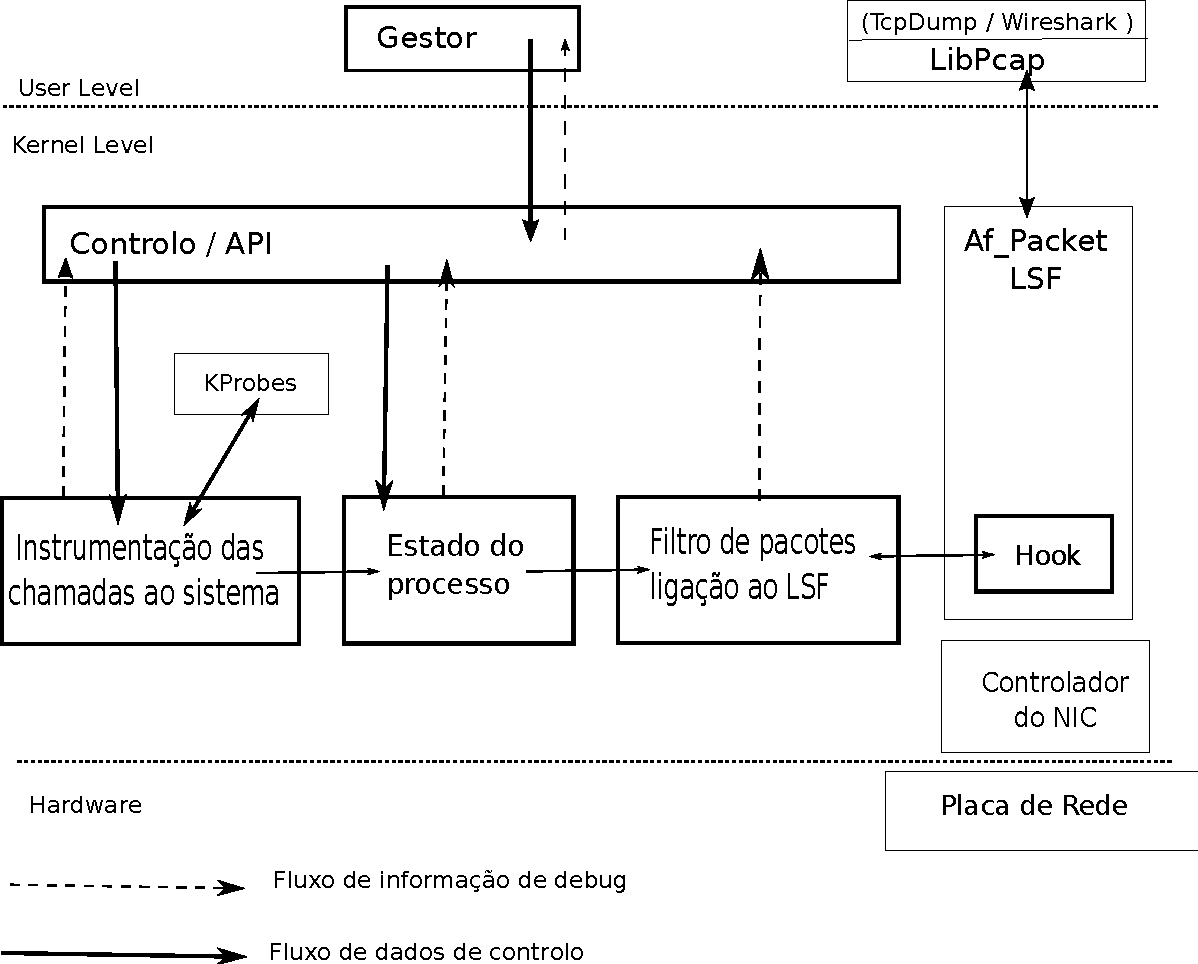
\includegraphics[scale=0.5]{interface.pdf} 
\caption{Arquitectura da solução}
\label{arquitectura}
\end{center}
\end{figure}


Este sistema permite que sejam capturados os pacotes de rede de um processo, sem que exista um conhecimento prévio sobre o(s) protocolo(s) ou portas utilizadas. A utilização de um sistema de instrumentação do núcleo foi necessária apenas para monitorizar as chamadas envolvendo \emph{sockets} e identificar o processo responsável, permitindo desta forma obter e manter permanentemente actualizada a informação sobre o estado respeitante ao processo alvo. De forma a minimizar a redução de desempenho, todo o sistema foi desenvolvido dentro do núcleo do \textit{Linux}, sem alterações nas interfaces já existentes.  Assim, ferramentas de façam uso da biblioteca \textit{LibPcap}, como o programa \textit{tcpdump} ou suas variantes, podem beneficiar desta extensão sem qualquer alteração e sem impacto relevante no seu desempenho.



\subsection*{Instrumentação das chamadas ao sistema de rede}
\label{sub:mon_syscalls}

Um ponto importante deste sistema, constituiu na garantia que todas as interacções desencadeadas por um processo com o exterior fossem detectadas. Para tal, foi necessário recorrer à monitorização das chamadas ao sistema de rede ao nível do Kernel, permitindo, assim, minimizar as cópias de dados e trocas de contexto. Tirando partido da utilização do sistema de monitorização KProbes foi possível realizar a monitorização sob o pequeno conjunto de chamadas ao sistema relevantes, nomeadamente: sendto, recvfrom, bind, accept, connect e close.
 Na realidade verificou-se a chamada ao sistema close, ao ser utilizada intensivamente por todo o sistema de ficheiros, poderia degradar desnecessariamente o desempenho. Desta forma, decidiu-se aplicar a monitorização à função sock\_close, garantindo apenas a monitorização das chamadas close sobre os sockets, reduzindo significativamente o número de eventos respeitantes à chamada ao sistema close.

\subsection*{Estado do processo}
\label{sub:data_repository}

O estado dos portos TCP e UDP em uso pelo processo alvo é mantido num repositório de dados, e permanentemente actualizado pelo módulo anterior. 
 A estrutura dados escolhida para o efeito, para produzir o repositório pretendido, baseia-se numa árvore \textit{Red and Black} já disponível no núcleo do sistema. O conteúdo de cada folha da árvore é uma estrutura com duas listas de elementos, cada uma contendo endereços IP utilizados pela aplicação. A chave de indexação das folhas é o número do porto, desta forma a àrvore poderá conter 65535 elementos. No pior caso a procura de um porto na àrvore necessitará de efectuar 16 iterações.
 \td{conteúdo? ip, interface, porto udp, porto tcp, etc??}
  O uso deste tipo de estrutura permite obter um bom compromisso entre o tempo de acesso à estrutura e a quantidade de memória utilizada.


\subsection*{Filtro de pacotes}
\label{sub:packet_filter}

A função de filtragem  implementada neste sistema assenta no estado do processo alvo, mantido pelos módulos anteriormente descritos.
Através da extensão do LSF com um hook, quando ligado, este invoca esta filtragem que devolve ao LSF se o pacote deve ser logo ignorado (não envolve nenhum dos portos do processo alvo) ou se se deve continuar a avaliar as restantes regras de filtragem definidas. Mantém-se assim a compatibilidade e continua-se a tirar partido dos benefícios da utilização do Linux Socket Filter.



\subsection*{Controlo e Informação}
\label{sub:data_information}

Para comunicar entre o sistema desenvolvido e uma aplicação monitorizadora foi necessário definir alguns ficheiros. Esta ficheiros estão apenas acessíveis ao utilizador \textit{root}, permitindo que outros utilizadores da máquina não consigam manipular o sistema de monitorização. Os ficheiros de controlo definidos foram \textit{option}, \textit{pid}, \textit{ppid} e \textit{tgid}. O primeiro ficheiro permite controlar a análise e a informação da àrvore, e os restantes são os identificadores do(s) processo(s), permitindo, em geral, monitorizar todos os processos pertencentes a um programa. Os ficheiros de informação foram definidos para obter estatísticas dos pacotes e das entradas/retornos das funções instrumentadas.

 \td{ Esta compreende três ficheiros . . . quais ? para quê? }

%%%%%%%%%%%%%%%%%
\subsection{Aplicação Monitora}
\label{sub:monitor_app}

Para poder efectuar alguns testes de avaliação foi criado uma aplicação em nível utilizador para poder lançar sob seu controlo a aplicação a ser monitorizada. Esta situação foi devida à necessidade de saber o momento em que se dá o inicio e o fim da aplicação, de forma a indicar ao sistema qual a aplicação a monitorizar e para poder obter o tempo de execução.

%%%%%%%%%%%%%%%%%%%


\section{Avaliação}
\label{sec:evaluation}

O sistema implementado foi avaliado funcionalmente através da utilização de protocolos \textit{ftp}\cite{ftp-proto} e \textit{http} \cite{HypTraPro--HTT}. Para tal, recorreu-se a um conjunto alargado de testes, tendo como objectivo não só observar o seu desempenho, como também, e mais importante, verificar a correcção do funcionamento e a sua capacidade de capturar todos os pacotes envolvidos nas comunicações de um processo alvo (e apenas esses pacotes). 

%Através destes conjunto de testes, foi possível efectuar a captura dos pacotes resultantes da transferência de um ficheiro, a partir de um servidor ftp ou http. 

De modo a realizar os testes de desempenho, foram utilizadas duas máquinas com interfaces de 100Mbits/s, ligadas directamente através de um cabo Ethernet cruzado. Uma das máquinas ficou responsável pela execução dos serviços \textit{ftp}, \textit{http} e \textit{iperf}.

\subsection{Avaliação Funcional}
A análise funcional foi efectuada por meio de programas simples, que desencadeiam chamadas sucessivas de criação de sockets e comunicação, obtendo-se o estado destes (portos e endereços) dentro do módulo do núcleo. Estes dados poderam ser confirmados através do sistema \textit{debugfs}, por consulta do ficheiro existente para esse efeito. Este ficheiro, quando acedido, contém toda a informação relativa aos portos e endereços em utilização por parte da aplicação monitorizada.
Deste modo, para obter um grau de comparação dos dados produzidos e validar esta análise, foi utilizada a ferramenta \textit{netstat}~\cite{netstat}, na qual indica os dados relativos aos portos e endereços utilizados pelos processos do sistema (esta ferramenta tira partido do sistema de ficheiros virtual \textit{ProcFs} ~\cite{procfskernel} para obter esses dados.
Para além desta análise, foi efectuada a confirmação da correcção de que todos os pacotes pertencentes às comunicações foram de facto obtidos. Esta confirmação foi efectuada através da captura utilizando o \textit{tcpdump} com o módulo activo, e verificado que todo o trafego respeitante ao protocolo (\textit{ftp} e \textit{http}) estava de facto capturado e correcto, não existindo mais fluxos pertencentes à captura.

\td{observação dos pacotes capturados com o tcpdump e wireshark e verificação de que a captura era correcta!!}

\subsection{Avaliação do desempenho}
Foram efectuados diversos testes para avaliação do overhwad introduzido por este sistema. Estes testes basearam-se na recepção ou transmissão de 1GigaByte de dados, por diferentes programas e protocolos, entre as duas máquinas conectadas directamente por interfaces de rede a 100 Mbit/s.

Na execução destes testes, foram executadas 10 iterações para cada experiência considerada, de modo a obter um valor médio com um desvio padrão aceitável (os resultados obtidos estão descritos nas tabelas \ref{tab:desempenho} e \ref{tab:overhead}).

\begin{table}
\begin{center}

\begin{tabular}{ | c | c | c | c |  }
\hline
Teste & \hspace {0.3cm} Original \hspace {0.3cm}& \hspace {0.2cm} Com TcpDump \hspace {0.2cm} & Com TcpDump e módulo \\
\hline
1GB - FTP & 91.8508	& 1.8500 & 91.8854 \\
1GB - HTTP & 91.6391 & 91.6472 & 91.6674 \\ 
%5GB - HTTP & 457.9506 & 457.9527 & 458.2059 \\
IPerf - 1GB TCP & 91.3790	& 91.2535	& 91.2672 \\
IPerf - 1GB UDP & 89.7975 & 89.8007 & 89.8464 \\
\hline
\hline
1GB HTTP 2 processos & 182.1573 & 188.7156 & 182.0161 \\
IPerf - 1GB UDP & 179.493 & 179.628 & 179.6369 \\
\hline
\end{tabular}
\caption{Tempos médios em segundos (s)}
\label{tab:desempenho}
\end{center}
\end{table}

Analisar estes dados .....

\begin{table}
\begin{center}

\begin{tabular}{ | c | c | c | c | }
\hline
Teste & TcpDump com módulo & Variação do TcpDump & \hspace {0.3cm} TcpDump \hspace {0.3cm}\\

\hline
1GB - FTP  & 0.0377 & 0.0385 & -0.0009 \\
1GB - HTTP &  0.0309 & 0.0220 & 0.0088 \\
%5GB - HTTP &  0.0557 & 0.0553 & 0.0005 \\
IPerf - 1GB TCP &  -0.1223 & 0.015 & 0.1373 \\
IPerf - 1GB UDP & 0.0545 & 0.0509 & 0.0036 \\
\hline
\hline
1GB HTTP 2 processos & -0.0775 & -3.5501 & 3.6003 \\
IPerf - 1GB UDP & 0.0802 & 0.005 & 0.0752 \\
\hline
\end{tabular}
\caption{Sobrecarga das transferências (valores em percentagem)}
\label{tab:overhead}
\end{center}
\end{table}


analisar estes dados ....

\subsubsection{Desempenho da estrutura de dados}
Para além das avaliações descritas anteriormente, tornou-se essencial analisar o comportamento da estrutura de dados utilizada para manter o “estado do processo”, de modo a verificar o compromisso entre o desempenho, a versatilidade e o espaço ocupado da mesma, sobre o sistema criado. Assim, para esta análise, foi elaborado um teste que usa o sistema de alta resolução de temporizadores (HRTimer) \cite{hrtimerKernel}, contido no núcleo do sistema de operação.

\begin{table}
\begin{center}

\begin{tabular}{ | l | c |  }
\hline
\hspace{1.2cm} Teste \hspace{1cm} & \hspace{1cm}Duração\hspace{1cm} \\
\hline
Adicionar 1 elemento & \\
\hline
Remove 1 elemento & \\
\hline
Adicionar 1024 elementos & 869 244\\
\hline
Remove 1024 elementos & 675 086\\
\hline

\hline
\end{tabular}
\caption{Tempos em nanosegundos}
\label{tab:tree_info}
\end{center}
\end{table}

\subsubsection{Desempenho do Sistema de instrumentação}
Sendo a instrumentação do sistema um ponto fundamental na execução da monitorização de uma aplicação, a análise ao seu comportamento é bastante importante, na medida em que é necessário verificar se a introdução deste tipo de sistemas, irá produzir uma elevada penalização sobre o sistema de operação. Tendo em conta que o sistema de instrumentação utilizado corresponde ao \textit{KProbes}, foi fundamental efectuar esses testes, de modo a garantir que tal factor não sucedia, através dos valores indicados em \cite{KProbeKernel}.

\begin{table}
\begin{center}

\begin{tabular}{ | c | c |  }
\hline
Teste & \hspace{1cm}Duração\hspace{1cm} \\
\hline
100 000 000 chamadas & \\
\hline
 & \\
\hline

\hline
\end{tabular}
\caption{Tempos em }
\label{tab:kprobes_info}
\end{center}
\end{table}


\section{Trabalho Relacionado}
\label{sec:related_work}


Este trabalho vem na sequência dos trabalhos efectuado por Nuno Farruca~\cite{Farruca:2009,duarte10}, que teve como objectivo monitorizar os processos de um sistema distribuído, tirando partido do libPCap e LSF existente em Linux. As dificuldades sentidas em obter apenas o trafego respeitante à aplicação sob monitorização levou a duas soluções. A primeira, monitorizarando o comportamento do processo através da criação de uma biblioteca que mapeia as funções sobre sockets da biblioteca de C \textit{LibC} de forma a obter os seus parâmetros e assim comunicar ao monitor quais dos pacotes capturados pelo PCap são ou não relevantes. Esta biblioteca é ligada aos processos da aplicação, no seu arranque, por definição da variável LD\_PRELOAD.
 Uma outra forma foi obter os dados dos sockets pertencentes aos processos alvo através de consultas periódicas do sistema de ficheiros virtual \textit{ProcFs} e executar também depois a filtragem de quais os pacotes dizem respeito à aplicação alvo.  Estas soluções sofrem de grandes problemas de desempenho além de, para a segunda solução, não oferecer garantias de que todo o tráfego relevante era mantido.

O trabalho~\cite{1688981} com o título \textit{Application-specific packet capturing using kernel probes}, efectuou uma monitorização, utilizando o sistema de instrumentação \textit{KProbes}, das funções de transmissão e recepção de dados dentro do núcleo do sistema. Desta forma é possível monitorizar os dados de um processo. Os dados recolhidos são analisados com o intuito de perceber se determinada porta e endereço são conhecidos e caso não sejam é adicionada a informação a uma tabela de dispersão utilizada para efectuar um novo filtro. O pacote capturado  é atrasado e re-injectado e forma a poder ser capturado pela biblioteca \textit{LibPCap} através do novo filtro.

\section{Conclusões}
\label{sec:conclusions}


\bibliographystyle{plain}
\bibliography{references}

\end{document}
